
During the dedicated experiment that took place in the SPS
in 2018 with the CCs, the measured emittance
growth was found to be a factor four (on average) lower than
expected from the theory (see Section~\ref{sec:meas_2018_vs_theory}). The reason for this discrepancy remained unresolved for some time, as detailed follow-up studies (see Chapter~\ref{Ch:investigating_discrepancy}) investigated and excluded a number of possible explanations for the discrepancy.
It was recently found, that the beam transverse impedance, which is not included in the theory~\cite{PhysRevSTAB.18.101001} used for the comparison with the measurements may impact the noise-induced emittance growth and explain the experimental observations. Here, the damping mechanism from the beam transverse impedance is investigated and discussed with detailed PyHEADTAIL simulations.

The structure of this chapter is as follows:




\section{SPS transverse impedance model}\label{sec:sps_impedance_model}
The PyHEADTAIL studies presented in this chapter are performed including the detailed transverse impedance model of the SPS machine~\cite{sps_impedance_model_git}. This model has been developed through a combination of theoretical computations, electromagentic simulations and was benchmarked with beam-based measurements~\cite{Salvant:1274254, Zannini:1561199, Salvant:1271349, Zannini:2141779}. 
It includes the contributions from all the individual elements in the SPS lattice i.e. the resistive wall, the indirect space charge, the kickers, the RF cavities (200\,MHz and 800\,MHz), the step transitions and the horizontal and vertical beam position monitors~\cite{Zannini:2141779}. The model needs to represent the global impedance of the full machine. Thus, the total impednace is obtained by summing up the impedance of each element weighted with the beta function at its location and by dividing the sum by the average beta function of the SPS. For the Q26 optics the average horizontal and vertical beta functions are 42.09\,m and 42.01\,m respectively.
%https://indico.cern.ch/event/299470/contributions/686509/attachments/564150/777102/LIUSPS_transverse_imp_5.pdf
% The Wall contribution included both the resistive wall and the indirect SC.
Figure~\ref{fig:sps_impedance_model_H_V} shows the complete transverse impedance model of the SPS machine with the disentangled dipolar (blue) and quadrupolar (orange) terms to be plotted seperetaly. 

% Plot figures: /eos/user/n/natriant/Project_thesis/plot_wakefields_impedances_SPS
\begin{figure}[!ht]
    \centering
    \begin{subfigure}[t]{0.45\textwidth}
        \centering
        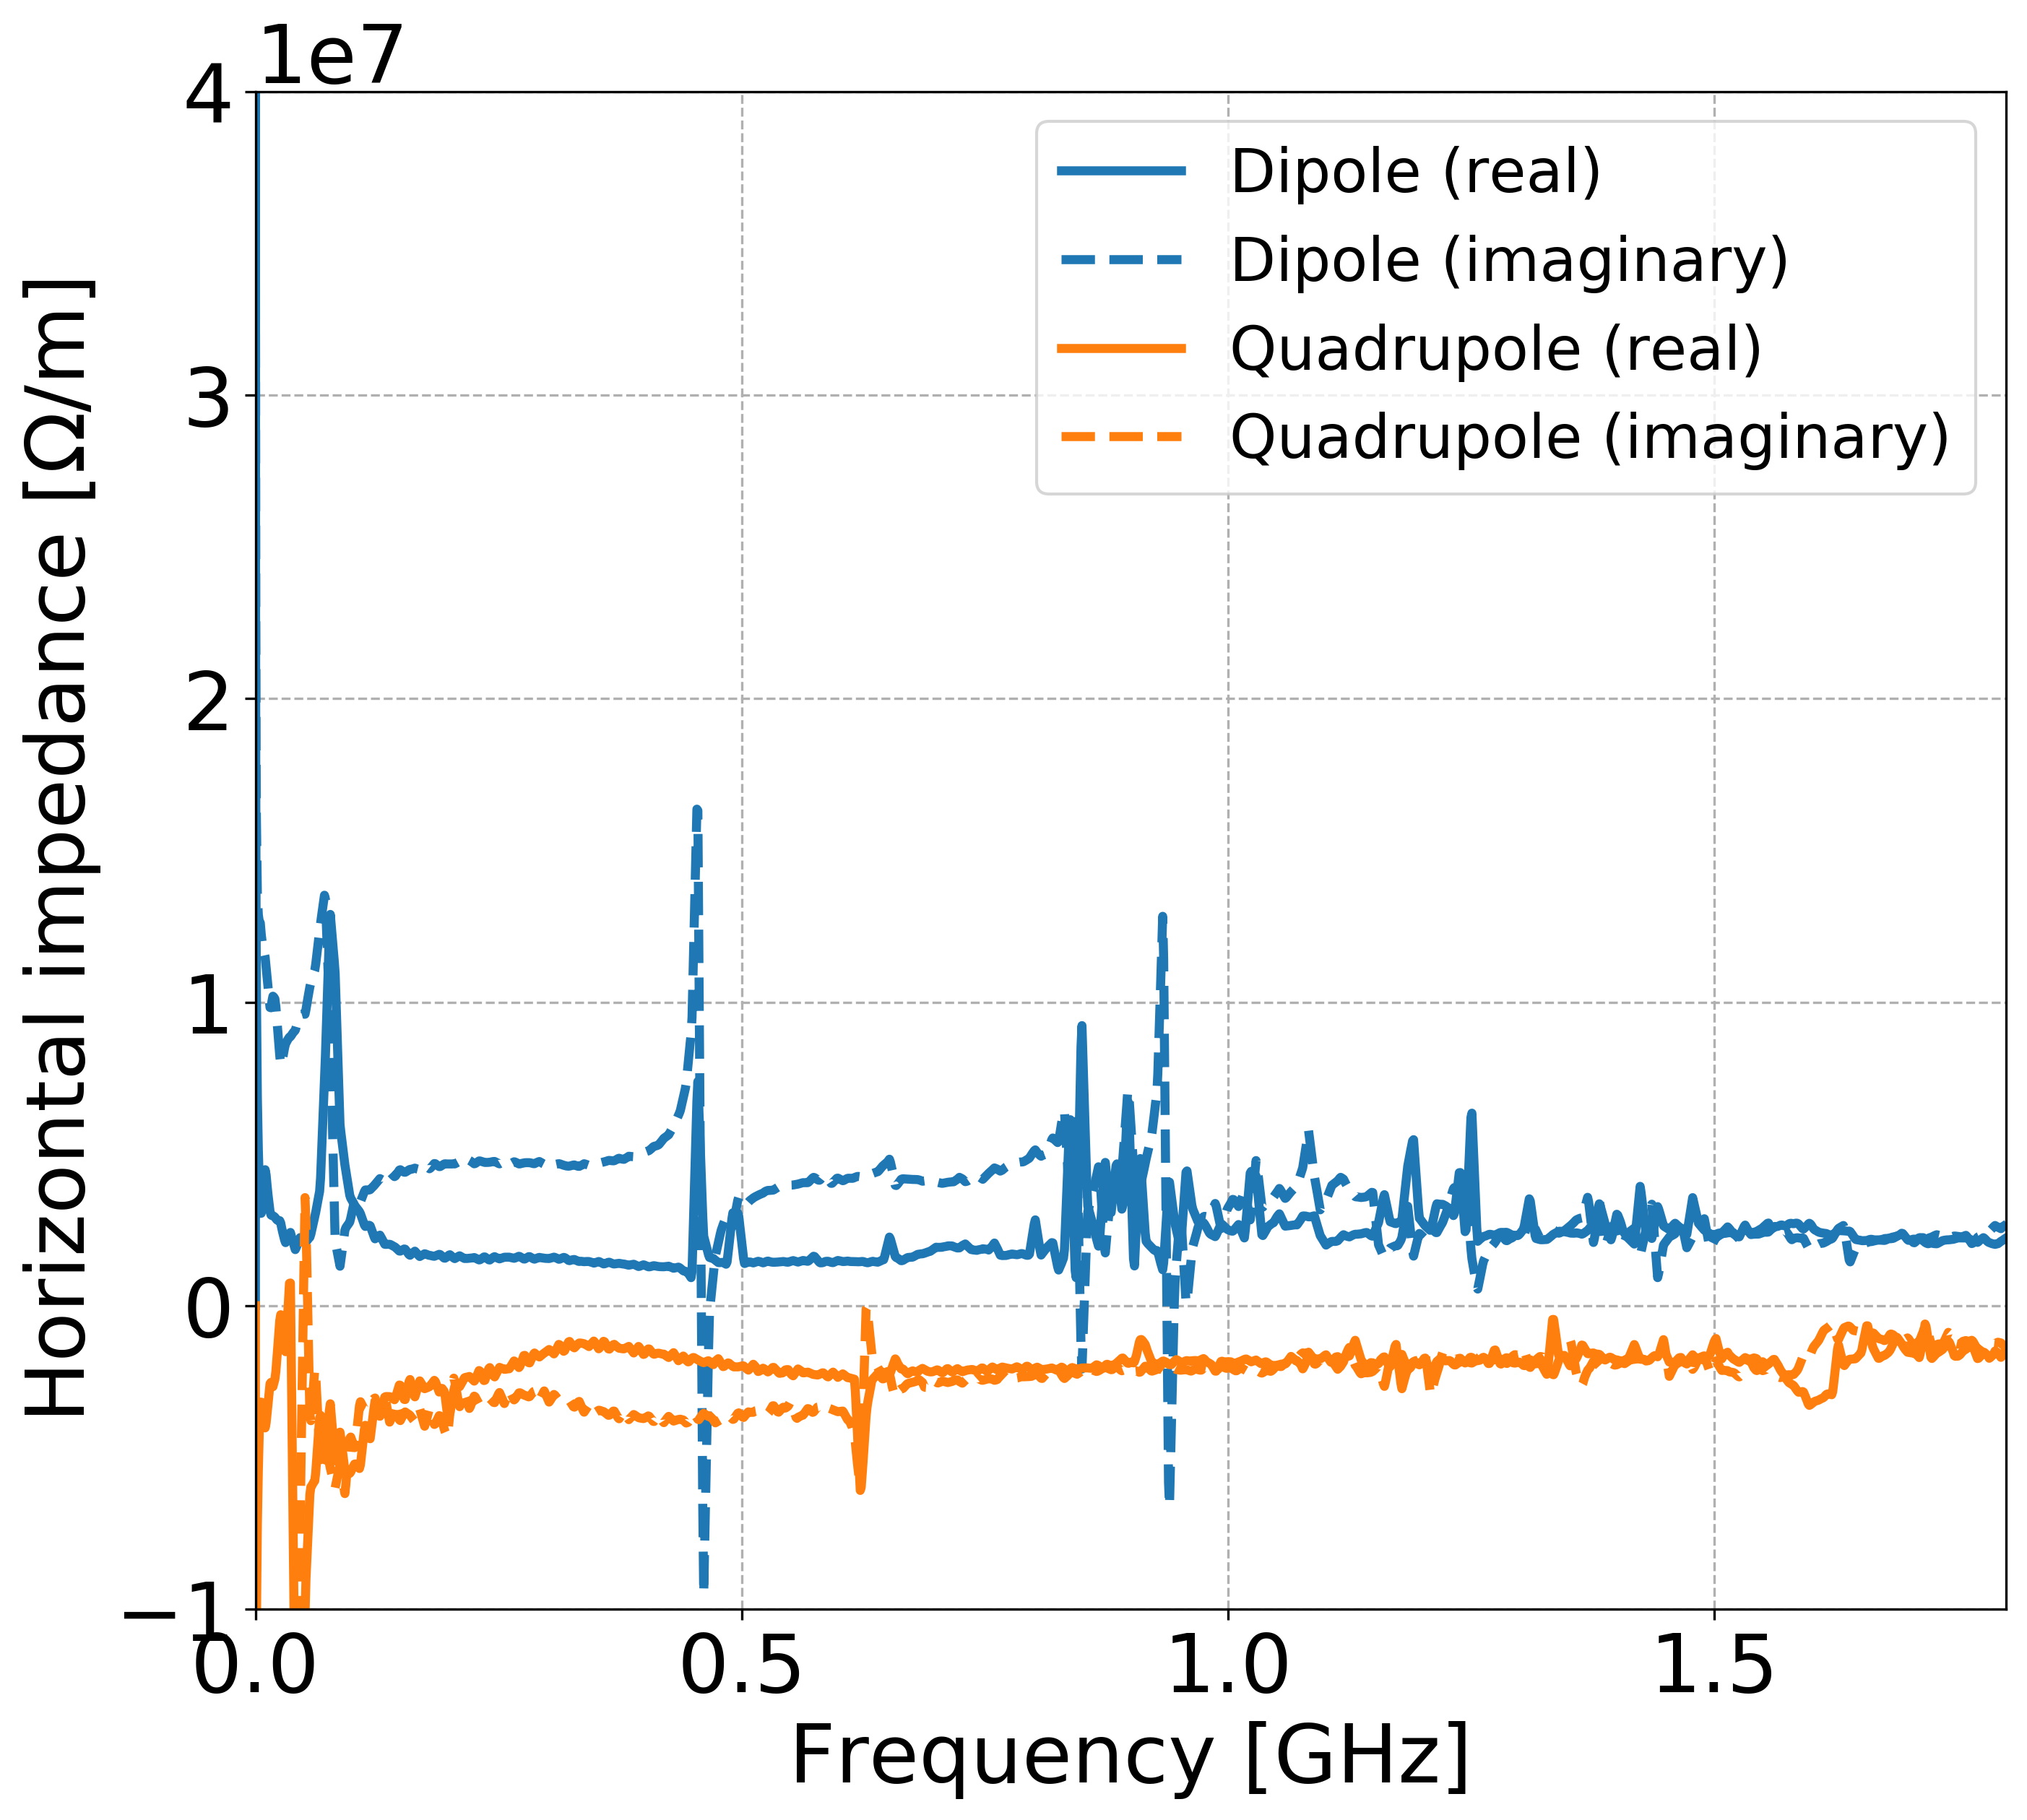
\includegraphics[width=1\textwidth]{images/Ch7/Q26_complete_SPS_model_impedance_H_plane.png}
        %\caption{$y=\sin(2 \pi f t),\ f=50$ Hz}
        %\label{fig:add_label_here}
    \end{subfigure}
    \hfill
    \begin{subfigure}[t]{0.45\textwidth}
        \centering
        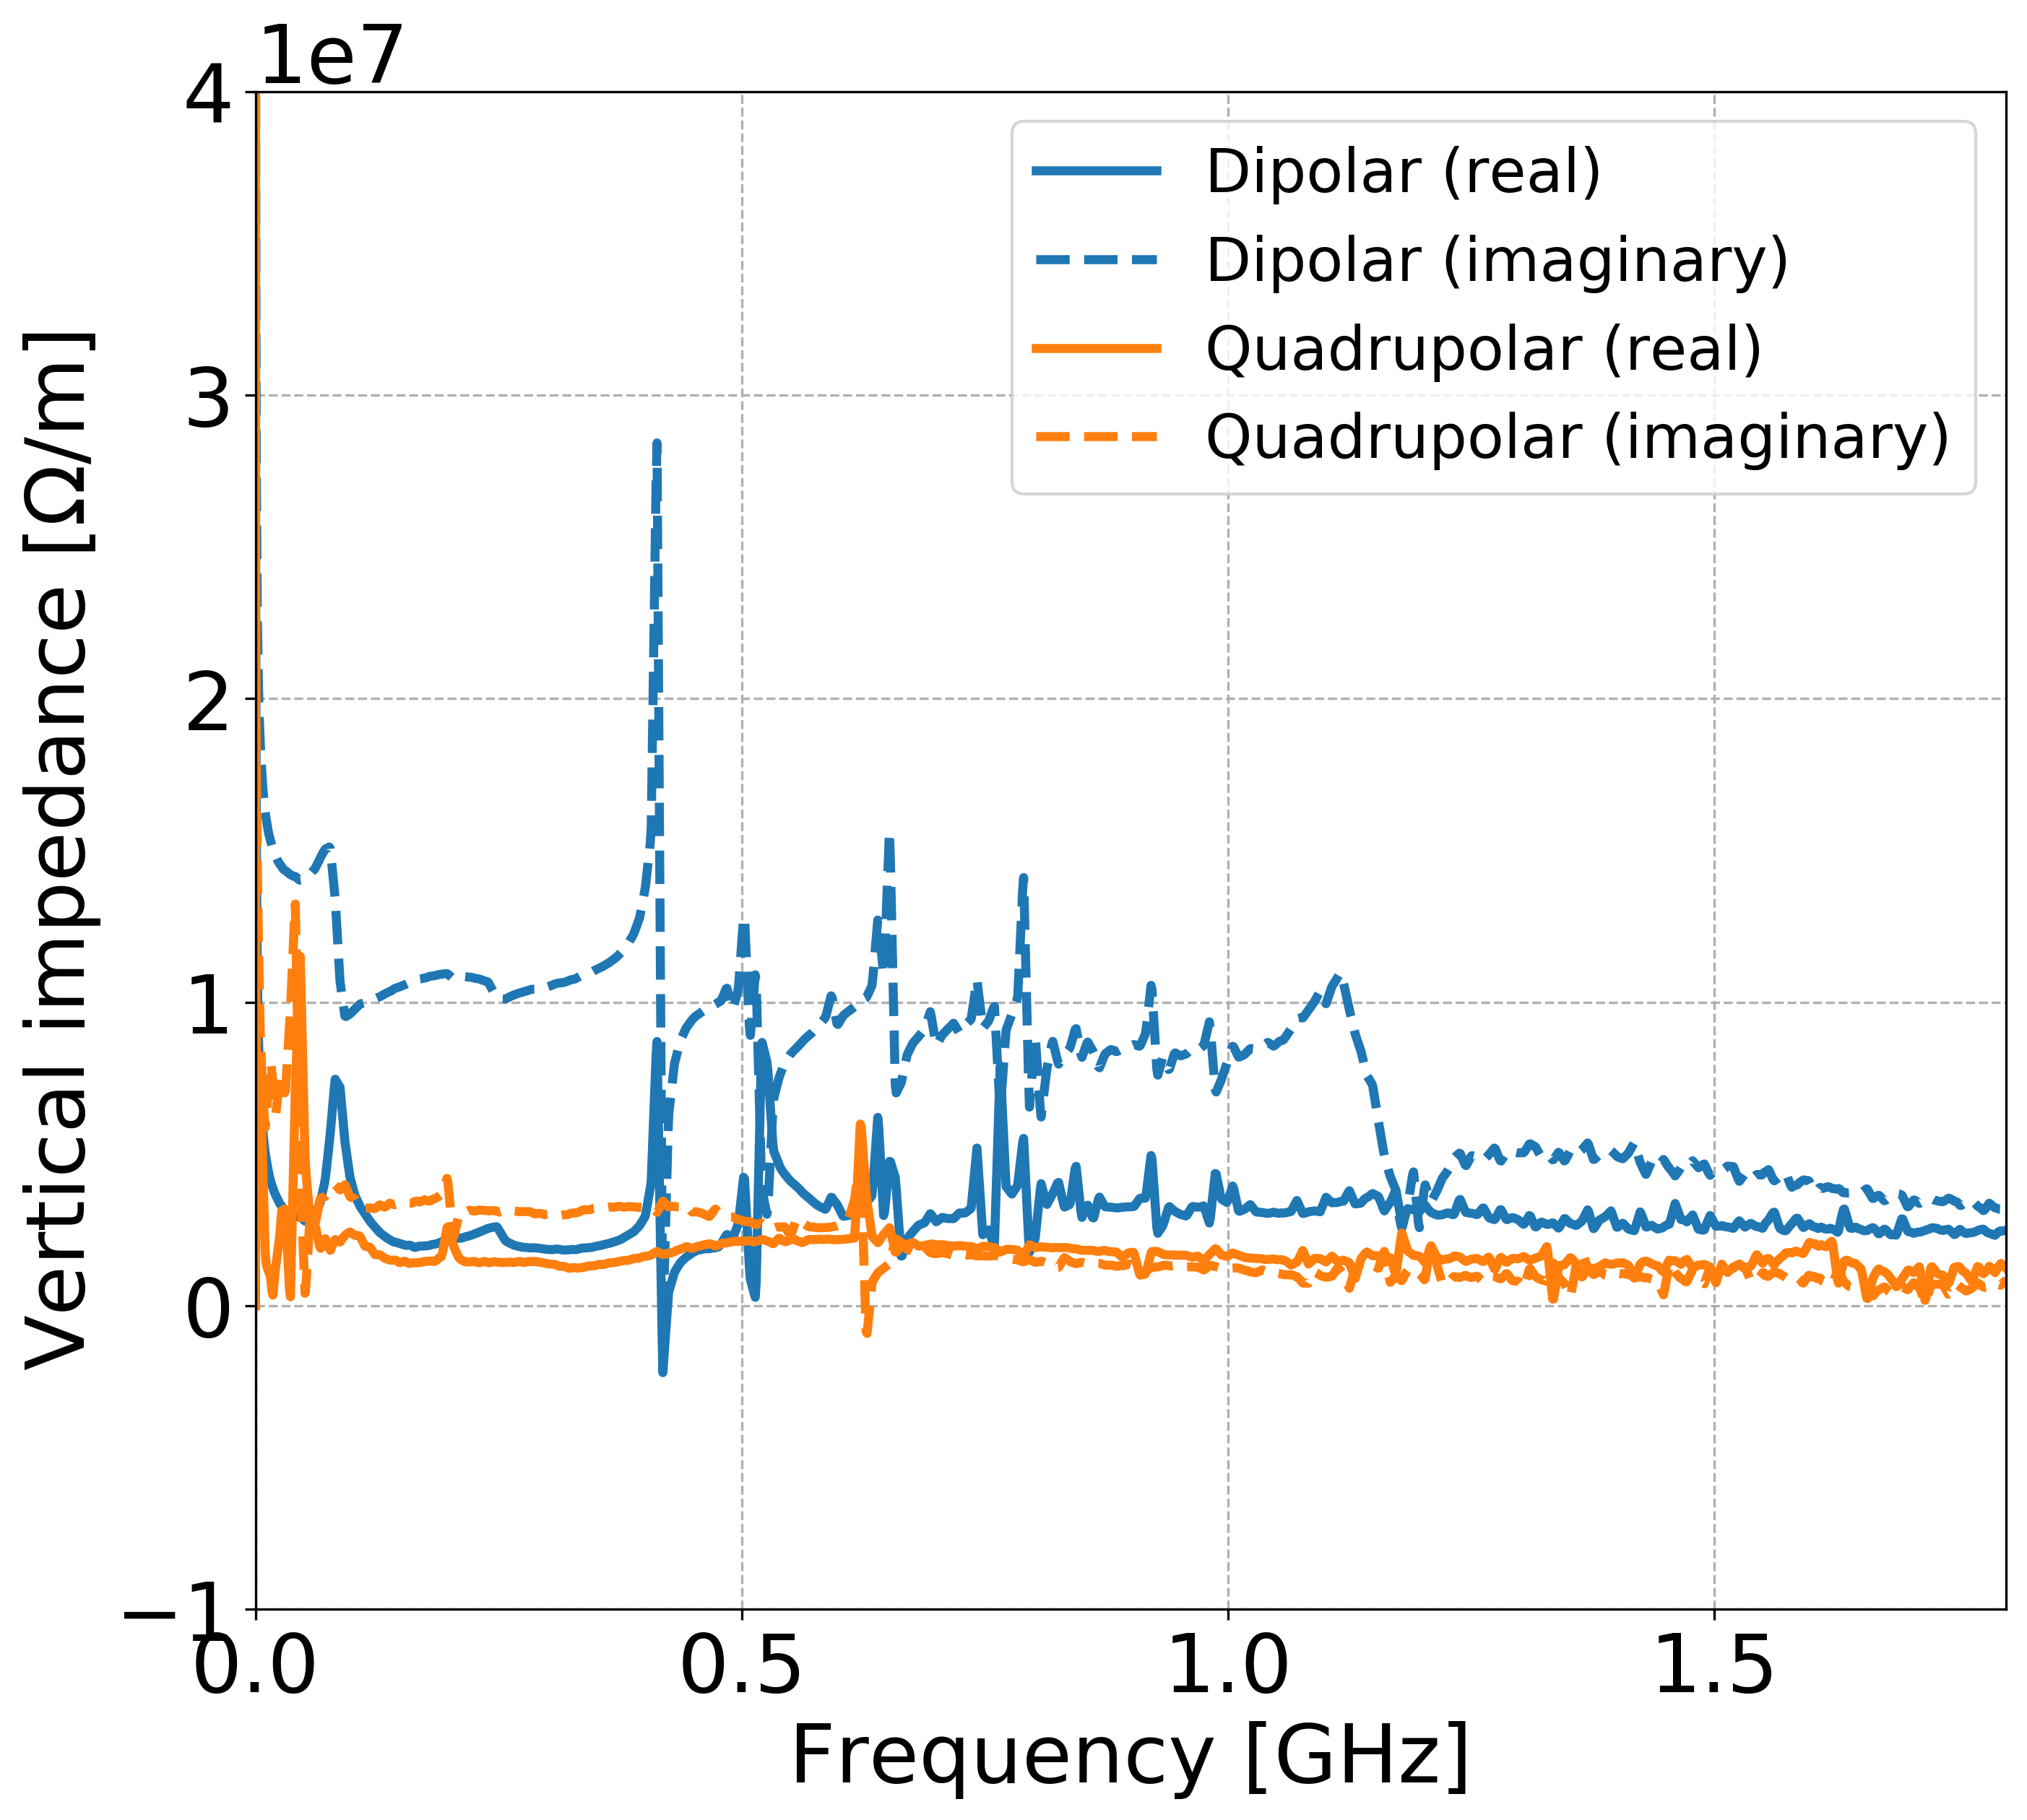
\includegraphics[width=1\textwidth]{images/Ch7/Q26_complete_SPS_model_impedance_V_plane.png}
        %\caption{Discrete Fourier transform}
        %\label{fig:add_label_here}
    \end{subfigure}
    \hfill
     \caption{Horizontal (left) and vertical (right) impedance model of the SPS.} % bunch passage
     \label{fig:sps_impedance_model_H_V}
 \end{figure}

 The contributions from the wall, the kickers and the step transitions are shown at the low freqencies (up to $\sim$ 0.4\,GHz). The impedance of the RF cavities and the beam position monitors (BPMs) corresponds results to the peaks observed between $\sim$ 0.4-1\,GHz. 
%https://indico.cern.ch/event/299470/contributions/686509/attachments/564150/777102/LIUSPS_transverse_imp_5.pdf


%For a clearer picture, it is worth mentioning that at low freqencies (up to $\sim$ 0.4\,GHz) the impedance is mainly from the wall the kickers and the step transitions. The peaks between $\sim$ 0.4-1\,GHz appear due to the RF cavities and the beam position monitors.
%https://indico.cern.ch/event/299470/contributions/686509/attachments/564150/777102/LIUSPS_transverse_imp_5.pdf

\subsection{Including the imepdance model in PyHEADTAIL simulations}

To simulate the impedance in 
In PyHEADTAIL the impedance is implemented in time domain i

In order to include the impedance effects in particle tracking simulations the real-values wakefields~\cite{sps_impedance_model_git} in time domain are used. As described in Section~\ref{sec:wakefields_theory} this corresponds to the inverse Fourier transformation of the complex-valued impedance in frequency domain. % more details in this procedure in the thesis of Benoit.
 The total transverse dipolar (blue) and quadrupolar (orange) wake functions for both planes of the SPS are plotted in Fig~\ref{fig:sps_wakefunctions_model_H_V}.

% Plot figures: /eos/user/n/natriant/Project_thesis/plot_wakefields_impedances_SPS
 \begin{figure}[!ht]
    \centering
    \begin{subfigure}[t]{0.45\textwidth}
        \centering
        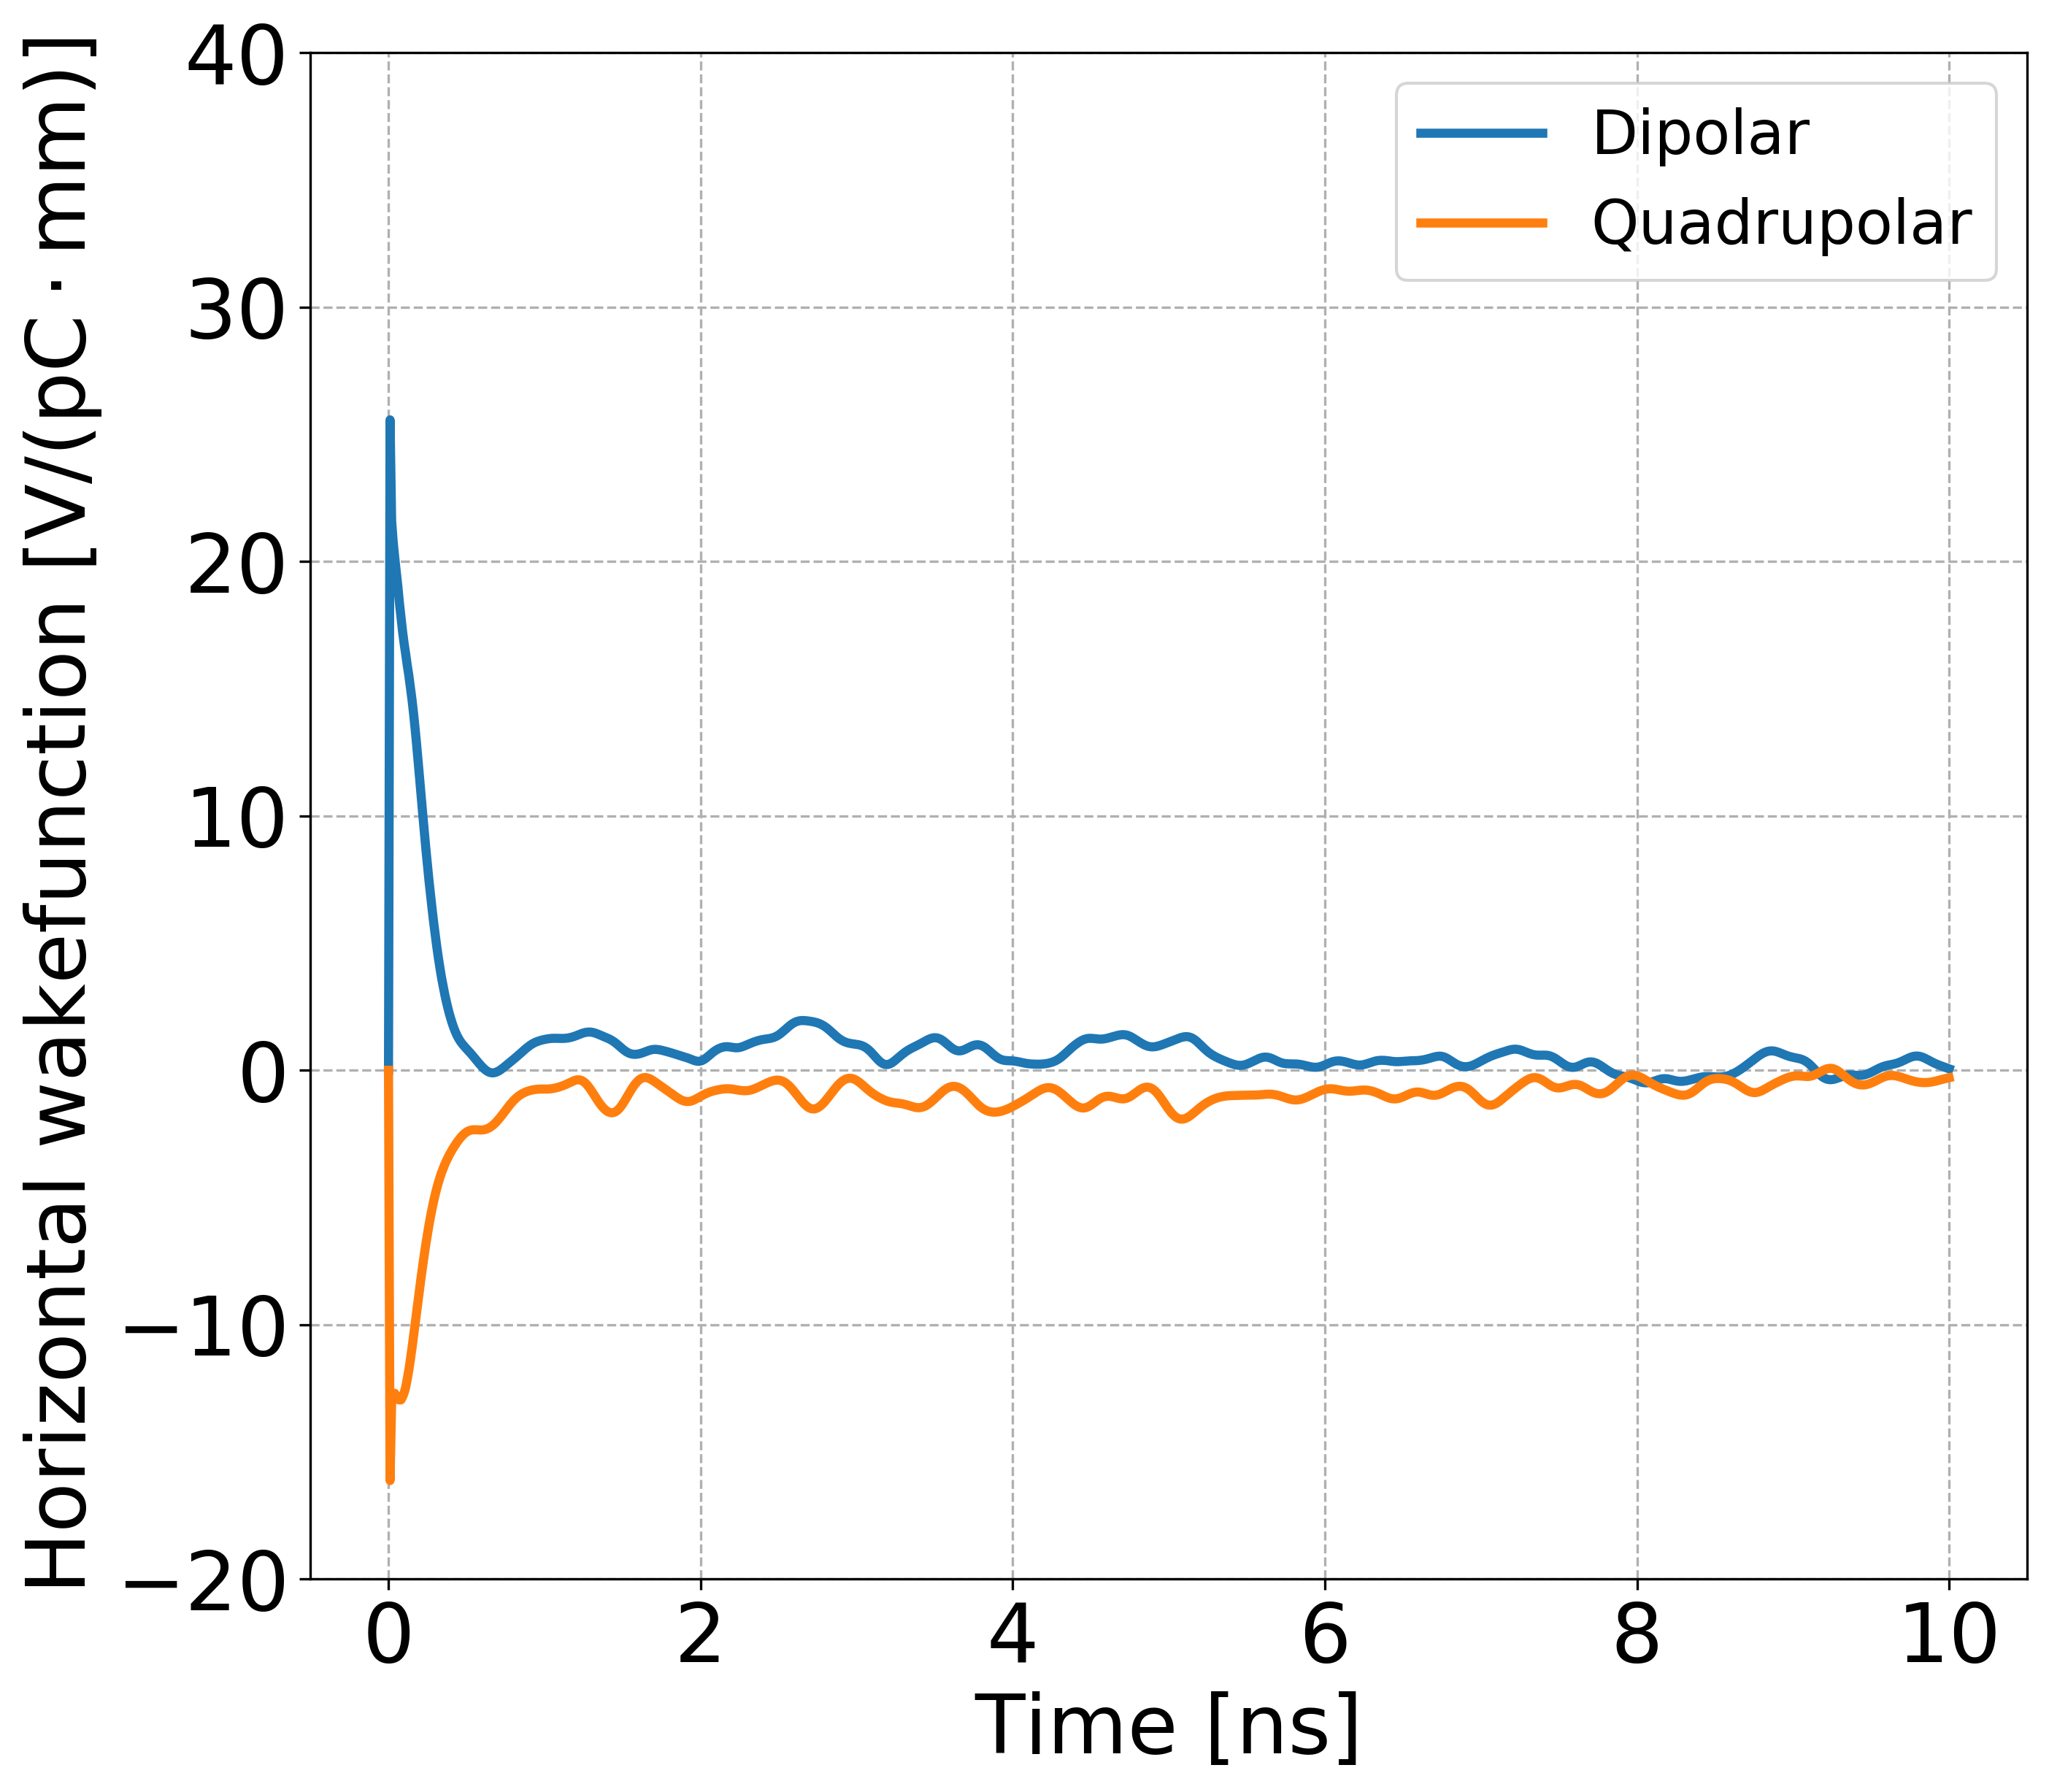
\includegraphics[width=1\textwidth]{images/Ch7/Q26_complete_SPS_model_wakefunctions_H_plane.png}
        %\caption{$y=\sin(2 \pi f t),\ f=50$ Hz}
        %\label{fig:add_label_here}
    \end{subfigure}
    \hfill
    \begin{subfigure}[t]{0.45\textwidth}
        \centering
        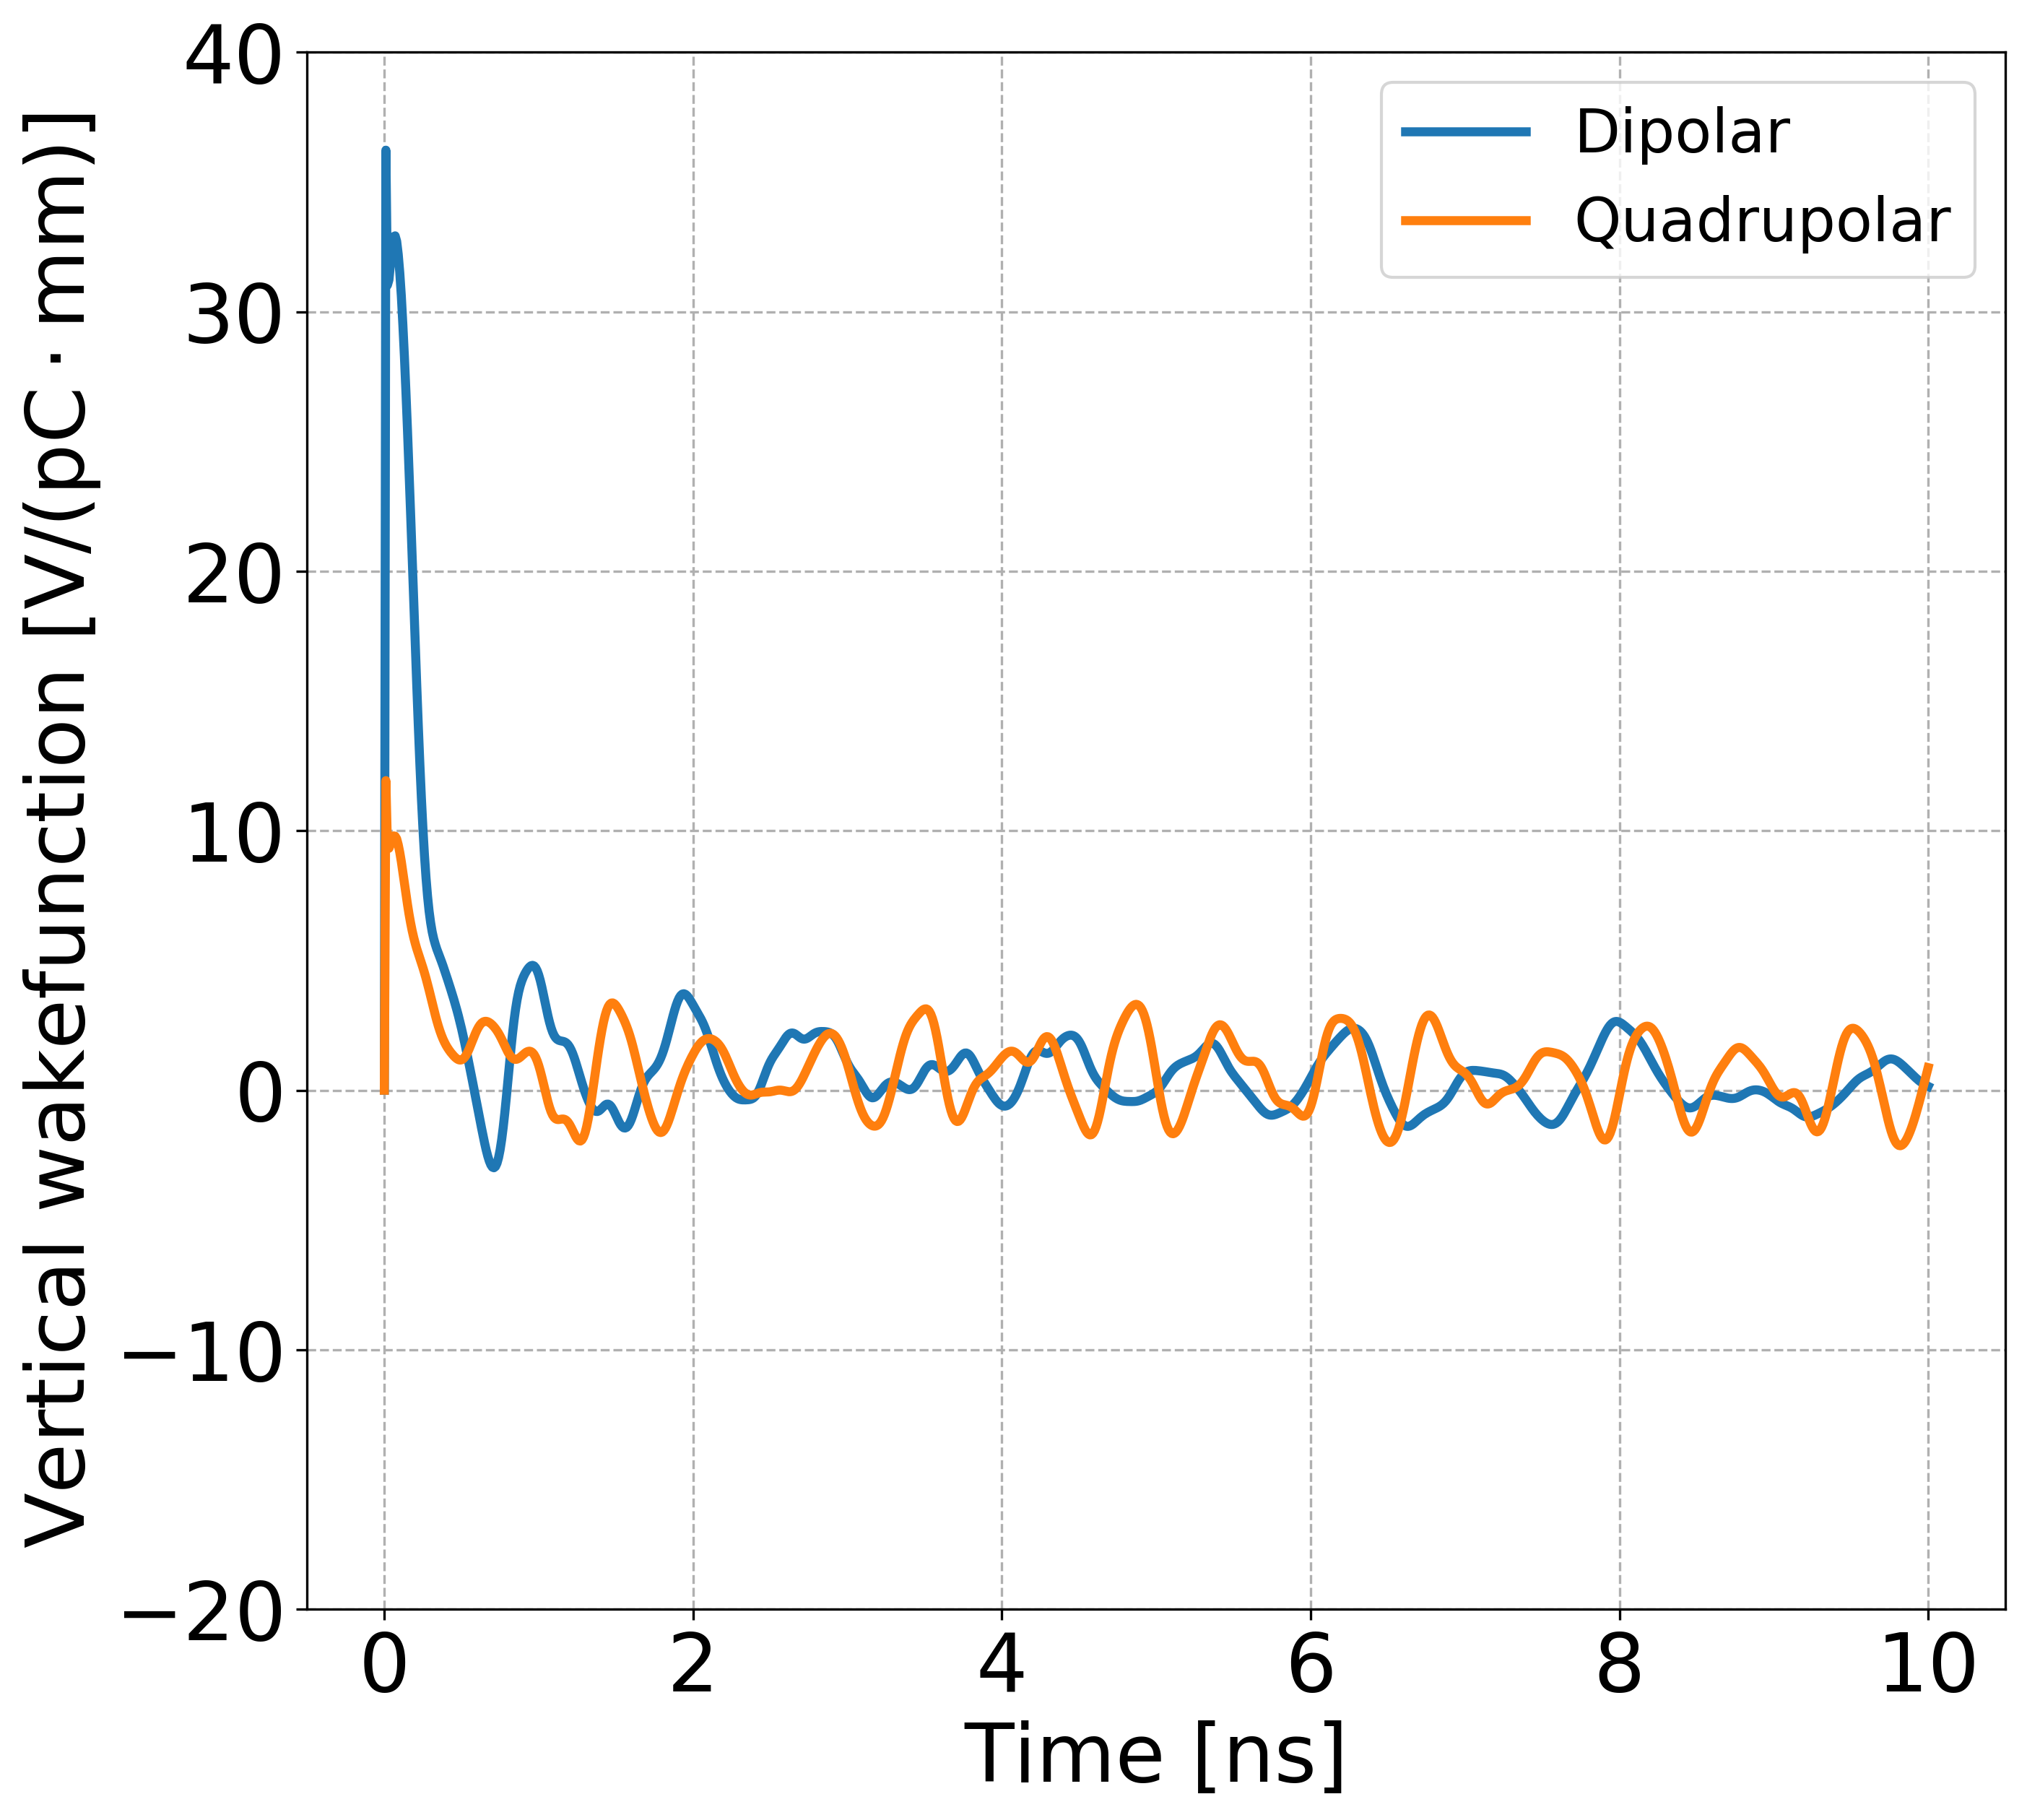
\includegraphics[width=1\textwidth]{images/Ch7/Q26_complete_SPS_model_wakefunctions_V_plane.png}
        %\caption{Discrete Fourier transform}
        %\label{fig:add_label_here}
    \end{subfigure}
    \hfill
     \caption{Horizontal (left) and vertical (right) wakefunctions of the SPS. For comparison the bunch length in the SPS CC experiments is $\sim$ 1.85\,ns (4$\mathrm{\sigma_t}$).} % bunch passage
     \label{fig:sps_wakefunctions_model_H_V}
 \end{figure}


% slide 9 https://accelconf.web.cern.ch/ipac2019/talks/weypls1_talk.pdf

PyHEADTAIL imports the wakefunctions (dipolar and quadrupolar term) for both transverse planes as tables.
The PyHEADTAIL assumes a constant average beta function around the machine.

We consider the wakes decay after one turn

Find a reference to refer to and thendescribe breifly here 1-2 sentences.Michael Scenk


% Carlo Zaninni thesis: s, it is important to have an accurate description of the wake at a
distance z significantly smaller than the RMS bunch-length, which means that the impedance
calculation needs to be accurate up to very high frequency (depending on the accelerator we
consider, from a few GHz to the range of THz). 

\subsection{Coherent tune shift with intensity}


\section{Simulations setup}




\section{First observations of emittance growth suppression from impedance}